\PassOptionsToPackage{unicode=true}{hyperref} % options for packages loaded elsewhere
\PassOptionsToPackage{hyphens}{url}
%
\documentclass[
  10pt,
  ignorenonframetext,
]{beamer}
\usepackage{pgfpages}
\setbeamertemplate{caption}[numbered]
\setbeamertemplate{caption label separator}{: }
\setbeamercolor{caption name}{fg=normal text.fg}
\beamertemplatenavigationsymbolsempty
% Prevent slide breaks in the middle of a paragraph:
\widowpenalties 1 10000
\raggedbottom
\setbeamertemplate{part page}{
  \centering
  \begin{beamercolorbox}[sep=16pt,center]{part title}
    \usebeamerfont{part title}\insertpart\par
  \end{beamercolorbox}
}
\setbeamertemplate{section page}{
  \centering
  \begin{beamercolorbox}[sep=12pt,center]{part title}
    \usebeamerfont{section title}\insertsection\par
  \end{beamercolorbox}
}
\setbeamertemplate{subsection page}{
  \centering
  \begin{beamercolorbox}[sep=8pt,center]{part title}
    \usebeamerfont{subsection title}\insertsubsection\par
  \end{beamercolorbox}
}
\AtBeginPart{
  \frame{\partpage}
}
\AtBeginSection{
  \ifbibliography
  \else
    \frame{\sectionpage}
  \fi
}
\AtBeginSubsection{
  \frame{\subsectionpage}
}
\usepackage{lmodern}
\usepackage{amssymb,amsmath}
\usepackage{ifxetex,ifluatex}
\ifnum 0\ifxetex 1\fi\ifluatex 1\fi=0 % if pdftex
  \usepackage[T1]{fontenc}
  \usepackage[utf8]{inputenc}
  \usepackage{textcomp} % provides euro and other symbols
\else % if luatex or xelatex
  \usepackage{unicode-math}
  \defaultfontfeatures{Scale=MatchLowercase}
  \defaultfontfeatures[\rmfamily]{Ligatures=TeX,Scale=1}
\fi
\usetheme[]{Warsaw}
\usecolortheme{whale}
\usefonttheme{structuresmallcapsserif}
% use upquote if available, for straight quotes in verbatim environments
\IfFileExists{upquote.sty}{\usepackage{upquote}}{}
\IfFileExists{microtype.sty}{% use microtype if available
  \usepackage[]{microtype}
  \UseMicrotypeSet[protrusion]{basicmath} % disable protrusion for tt fonts
}{}
\makeatletter
\@ifundefined{KOMAClassName}{% if non-KOMA class
  \IfFileExists{parskip.sty}{%
    \usepackage{parskip}
  }{% else
    \setlength{\parindent}{0pt}
    \setlength{\parskip}{6pt plus 2pt minus 1pt}}
}{% if KOMA class
  \KOMAoptions{parskip=half}}
\makeatother
\usepackage{xcolor}
\IfFileExists{xurl.sty}{\usepackage{xurl}}{} % add URL line breaks if available
\IfFileExists{bookmark.sty}{\usepackage{bookmark}}{\usepackage{hyperref}}
\hypersetup{
  pdftitle={A1 Getting started with R},
  pdfauthor={Jan-Philipp Kolb},
  pdfborder={0 0 0},
  breaklinks=true}
\urlstyle{same}  % don't use monospace font for urls
\newif\ifbibliography
\usepackage{color}
\usepackage{fancyvrb}
\newcommand{\VerbBar}{|}
\newcommand{\VERB}{\Verb[commandchars=\\\{\}]}
\DefineVerbatimEnvironment{Highlighting}{Verbatim}{commandchars=\\\{\}}
% Add ',fontsize=\small' for more characters per line
\usepackage{framed}
\definecolor{shadecolor}{RGB}{48,48,48}
\newenvironment{Shaded}{\begin{snugshade}}{\end{snugshade}}
\newcommand{\AlertTok}[1]{\textcolor[rgb]{1.00,0.81,0.69}{#1}}
\newcommand{\AnnotationTok}[1]{\textcolor[rgb]{0.50,0.62,0.50}{\textbf{#1}}}
\newcommand{\AttributeTok}[1]{\textcolor[rgb]{0.80,0.80,0.80}{#1}}
\newcommand{\BaseNTok}[1]{\textcolor[rgb]{0.86,0.64,0.64}{#1}}
\newcommand{\BuiltInTok}[1]{\textcolor[rgb]{0.80,0.80,0.80}{#1}}
\newcommand{\CharTok}[1]{\textcolor[rgb]{0.86,0.64,0.64}{#1}}
\newcommand{\CommentTok}[1]{\textcolor[rgb]{0.50,0.62,0.50}{#1}}
\newcommand{\CommentVarTok}[1]{\textcolor[rgb]{0.50,0.62,0.50}{\textbf{#1}}}
\newcommand{\ConstantTok}[1]{\textcolor[rgb]{0.86,0.64,0.64}{\textbf{#1}}}
\newcommand{\ControlFlowTok}[1]{\textcolor[rgb]{0.94,0.87,0.69}{#1}}
\newcommand{\DataTypeTok}[1]{\textcolor[rgb]{0.87,0.87,0.75}{#1}}
\newcommand{\DecValTok}[1]{\textcolor[rgb]{0.86,0.86,0.80}{#1}}
\newcommand{\DocumentationTok}[1]{\textcolor[rgb]{0.50,0.62,0.50}{#1}}
\newcommand{\ErrorTok}[1]{\textcolor[rgb]{0.76,0.75,0.62}{#1}}
\newcommand{\ExtensionTok}[1]{\textcolor[rgb]{0.80,0.80,0.80}{#1}}
\newcommand{\FloatTok}[1]{\textcolor[rgb]{0.75,0.75,0.82}{#1}}
\newcommand{\FunctionTok}[1]{\textcolor[rgb]{0.94,0.94,0.56}{#1}}
\newcommand{\ImportTok}[1]{\textcolor[rgb]{0.80,0.80,0.80}{#1}}
\newcommand{\InformationTok}[1]{\textcolor[rgb]{0.50,0.62,0.50}{\textbf{#1}}}
\newcommand{\KeywordTok}[1]{\textcolor[rgb]{0.94,0.87,0.69}{#1}}
\newcommand{\NormalTok}[1]{\textcolor[rgb]{0.80,0.80,0.80}{#1}}
\newcommand{\OperatorTok}[1]{\textcolor[rgb]{0.94,0.94,0.82}{#1}}
\newcommand{\OtherTok}[1]{\textcolor[rgb]{0.94,0.94,0.56}{#1}}
\newcommand{\PreprocessorTok}[1]{\textcolor[rgb]{1.00,0.81,0.69}{\textbf{#1}}}
\newcommand{\RegionMarkerTok}[1]{\textcolor[rgb]{0.80,0.80,0.80}{#1}}
\newcommand{\SpecialCharTok}[1]{\textcolor[rgb]{0.86,0.64,0.64}{#1}}
\newcommand{\SpecialStringTok}[1]{\textcolor[rgb]{0.80,0.58,0.58}{#1}}
\newcommand{\StringTok}[1]{\textcolor[rgb]{0.80,0.58,0.58}{#1}}
\newcommand{\VariableTok}[1]{\textcolor[rgb]{0.80,0.80,0.80}{#1}}
\newcommand{\VerbatimStringTok}[1]{\textcolor[rgb]{0.80,0.58,0.58}{#1}}
\newcommand{\WarningTok}[1]{\textcolor[rgb]{0.50,0.62,0.50}{\textbf{#1}}}
\usepackage{longtable,booktabs}
\usepackage{caption}
% These lines are needed to make table captions work with longtable:
\makeatletter
\def\fnum@table{\tablename~\thetable}
\makeatother
\usepackage{graphicx,grffile}
\makeatletter
\def\maxwidth{\ifdim\Gin@nat@width>\linewidth\linewidth\else\Gin@nat@width\fi}
\def\maxheight{\ifdim\Gin@nat@height>\textheight\textheight\else\Gin@nat@height\fi}
\makeatother
% Scale images if necessary, so that they will not overflow the page
% margins by default, and it is still possible to overwrite the defaults
% using explicit options in \includegraphics[width, height, ...]{}
\setkeys{Gin}{width=\maxwidth,height=\maxheight,keepaspectratio}
\setlength{\emergencystretch}{3em}  % prevent overfull lines
\providecommand{\tightlist}{%
  \setlength{\itemsep}{0pt}\setlength{\parskip}{0pt}}
\setcounter{secnumdepth}{-2}

% set default figure placement to htbp
\makeatletter
\def\fps@figure{htbp}
\makeatother


\title{A1 Getting started with R}
\author{Jan-Philipp Kolb}
\date{10 Januar, 2020}

\begin{document}
\frame{\titlepage}

\begin{frame}{\href{http://uc-r.github.io/data_wrangling/week-1}{COURSE
OBJECTIVES}}
\protect\hypertarget{course-objectives}{}

\begin{itemize}
\tightlist
\item
  Perform your data analysis in a literate programming environment
\item
  Import and manage structured and unstructured data
\item
  Manipulate, transform, and summarize your data
\item
  Join disparate data sources
\item
  Methodically explore and visualize your data
\item
  Perform iterative functions
\item
  Write your own functions
\end{itemize}

\ldots{} all with R!

\end{frame}

\begin{frame}{Introduction round}
\protect\hypertarget{introduction-round}{}

\begin{block}{Please tell us shortly\ldots{}}

\begin{itemize}
\tightlist
\item
  Where are you from? What are you studying/working?
\item
  What is your experience level in R/other programming languages?
\item
  What are your expectations of this course?
\item
  Where do you think you can use R in the future?
\end{itemize}

\end{block}

\end{frame}

\begin{frame}{Preliminaries}
\protect\hypertarget{preliminaries}{}

\begin{itemize}
\tightlist
\item
  Usually we have big differences in knowledge and abilities of the
  participants - please tell, if it is too fast or slow.
\item
  We have lots of hands-on coding
  \href{http://web.math.ku.dk/~helle/R-intro/exercises.pdf}{\textbf{exercises}}
  - later you can only learn on your own
\item
  We have many \href{https://www.showmeshiny.com/}{\textbf{examples}} -
  try them
\item
  If there are questions - always ask
\item
  R is more fun together - ask your neighbor - strong proponent of
  collaborative work!
\end{itemize}

\end{frame}

\begin{frame}{Sources of this course}
\protect\hypertarget{sources-of-this-course}{}

\begin{block}{Sources for figures, text, exercises etc:}

\begin{itemize}
\tightlist
\item
  If the source is a website, the links are often in the header or in
  bold somewhere on the slide.
\item
  At the end of a chapter, we often have additional links to read on.
\item
  Please ask us, if something is unclear.
\end{itemize}

\end{block}

\end{frame}

\begin{frame}{Reasons for using R\ldots{}}
\protect\hypertarget{reasons-for-using-r}{}

\begin{itemize}
\tightlist
\item
  \ldots{} because it is an
  \href{https://stackoverflow.com/questions/1546583/what-is-the-definition-of-an-open-source-programming-language}{\textbf{open
  source language}}
\item
  \ldots{} outstanding graphs -
  \href{http://matthewlincoln.net/2014/12/20/adjacency-matrix-plots-with-r-and-ggplot2.html}{\textbf{graphics}},
  \href{https://www.r-bloggers.com/3d-plots-with-ggplot2-and-plotly\%20/}{\textbf{graphics}},
  \href{https://procomun.wordpress.com/2011/03/18/splomr/}{\textbf{graphics}}
\item
  \ldots{} relates to other languages -
  \href{https://github.com/Japhilko/RInterfaces}{\textbf{R can be used
  in combination with other programs}} -
  e.g.~\href{https://github.com/Japhilko/RInterfaces/blob/master/slides/Datenimport.md}{\textbf{data
  linking}}
\item
  \ldots{}R can be used
  \href{https://cran.r-project.org/web/packages/MplusAutomation/index.html}{\textbf{for
  automation}}
\item
  \ldots{} Vast Community -
  \href{https://www.r-bloggers.com/}{\textbf{you can use the
  intelligence of other people ;-)}}
\item
  \ldots{}
\end{itemize}

\end{frame}

\begin{frame}{Advantages of R}
\protect\hypertarget{advantages-of-r}{}

\begin{itemize}
\tightlist
\item
  R can be downloaded for
  \href{http://mirrors.softliste.de/cran/}{\textbf{free}}.
\end{itemize}


\includegraphics{figure/forfree.PNG}

\begin{itemize}
\item
  R is a
  \href{https://en.wikipedia.org/wiki/Scripting_language}{\textbf{scripting
  language}}
\item
  R is becoming more
  \href{https://twitter.com/josiahjdavis/status/559778930476220418}{\textbf{popular}}
\item
  \href{http://www.sr.bham.ac.uk/~ajrs/R/r-gallery.html}{\textbf{Good}}
  possibilities for
  \href{http://research.stowers.org/mcm/efg/R/}{\textbf{visualization}}
\end{itemize}

\end{frame}

\begin{frame}{R can be used in combination\ldots{}}
\protect\hypertarget{r-can-be-used-in-combination}{}


\includegraphics{figure/Rinterfaces.PNG}

\begin{itemize}
\tightlist
\item
  Interface to:
  \href{https://cran.r-project.org/web/packages/reticulate/vignettes/calling_python.html}{\textbf{Python}},
  \href{https://www.springer.com/de/book/9781441900517}{\textbf{Excel}},
  \href{https://www.ibm.com/support/knowledgecenter/en/SSFUEU_7.2.0/com.ibm.swg.ba.cognos.op_capmod_ig.7.2.0.doc/t_essentials_for_r_statistics.html}{\textbf{SPSS}},
  \href{https://cran.r-project.org/web/packages/SASmixed/index.html}{\textbf{SAS}},
  \href{https://cran.r-project.org/web/packages/RStata/index.html}{\textbf{Stata}}
\end{itemize}

\end{frame}

\begin{frame}{\href{https://gallery.shinyapps.io/cran-gauge/}{\textbf{The
popularity of R-packages}}}
\protect\hypertarget{the-popularity-of-r-packages}{}

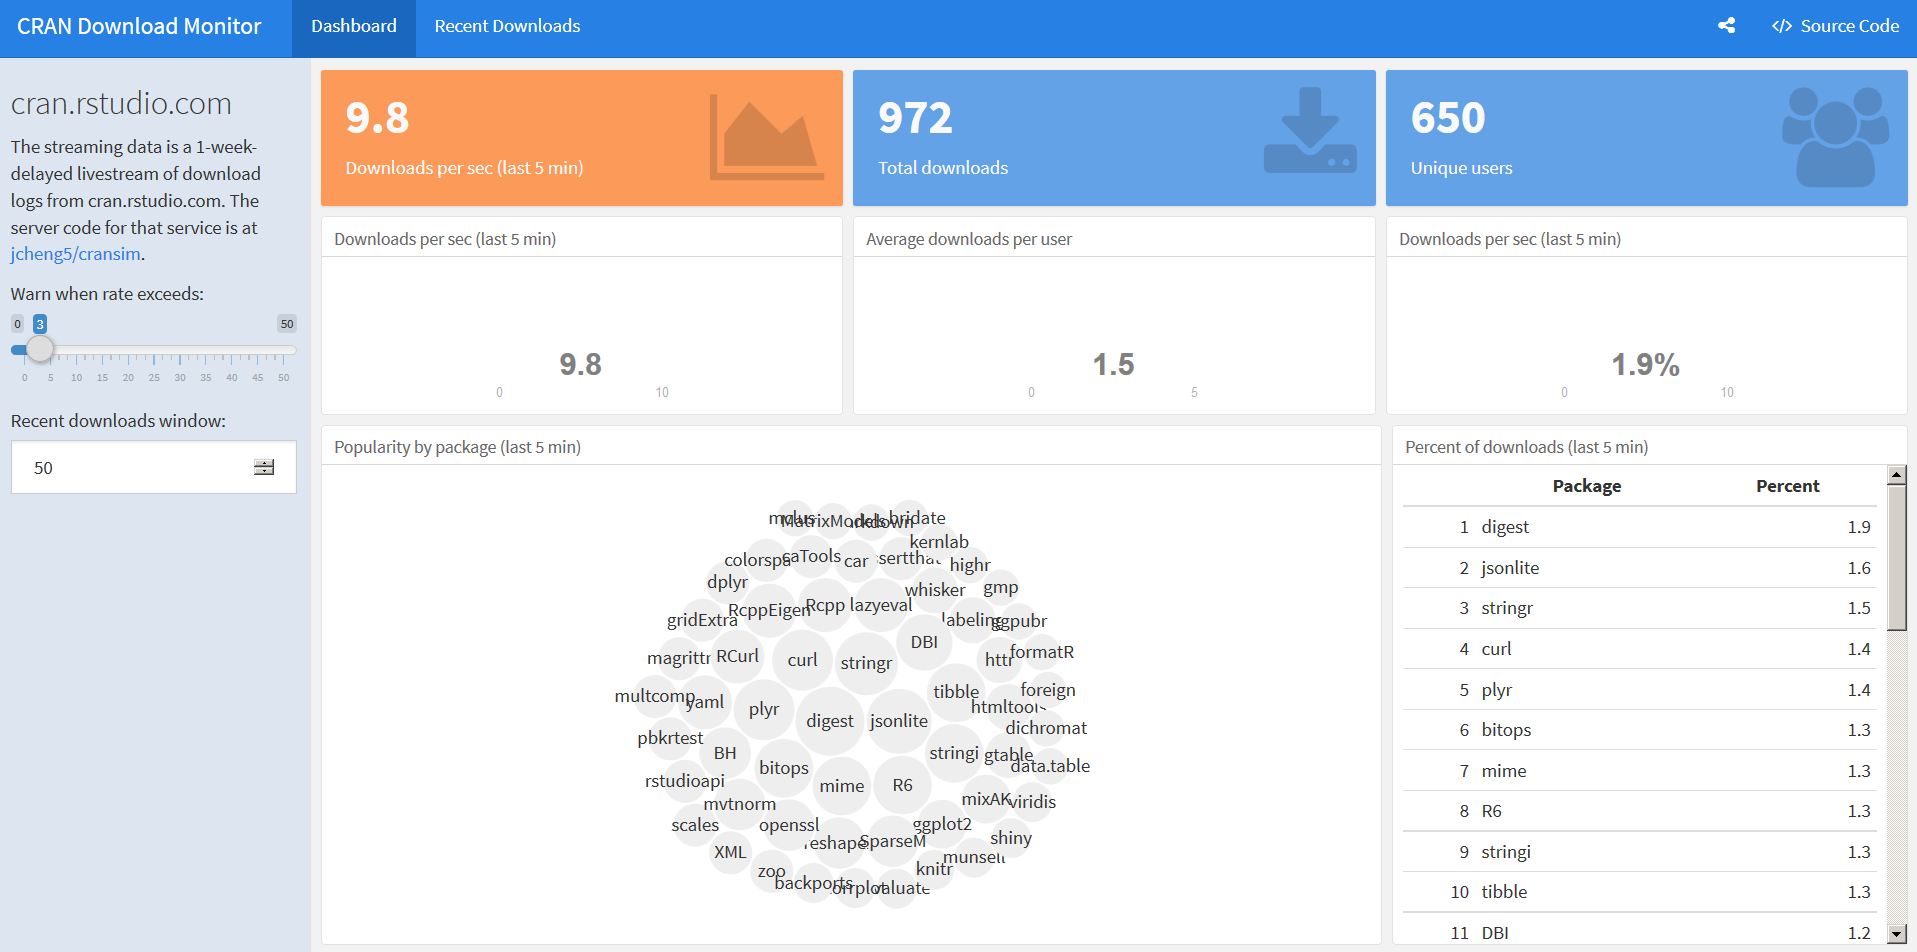
\includegraphics{figure/CRANdownloads.PNG}

\end{frame}

\begin{frame}{Download R:}
\protect\hypertarget{download-r}{}

\url{http://www.r-project.org/}

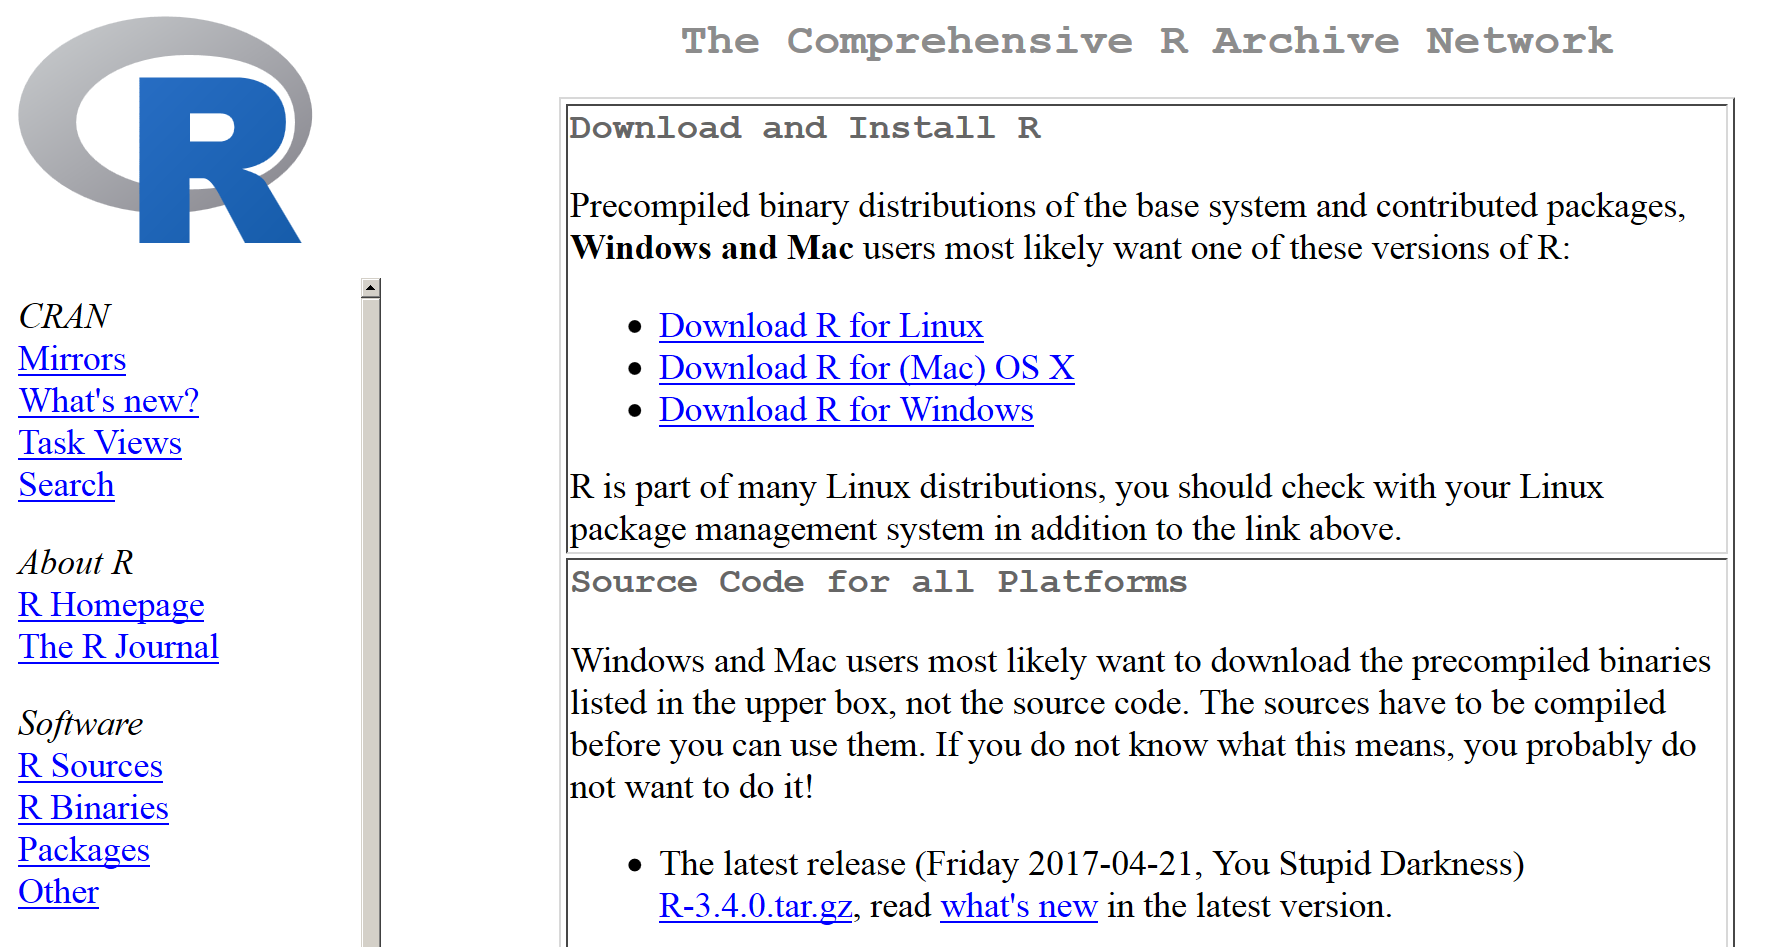
\includegraphics{figure/CRAN1picture.PNG}

\end{frame}

\begin{frame}{Open Source Programm R}
\protect\hypertarget{open-source-programm-r}{}

\begin{itemize}
\tightlist
\item
  R is a free, non-commercial implementation of the S programming
  language (by AT\&T Bell Laboratories)
\item
  Free participation - modular structure
\end{itemize}

\begin{block}{This is base R:}

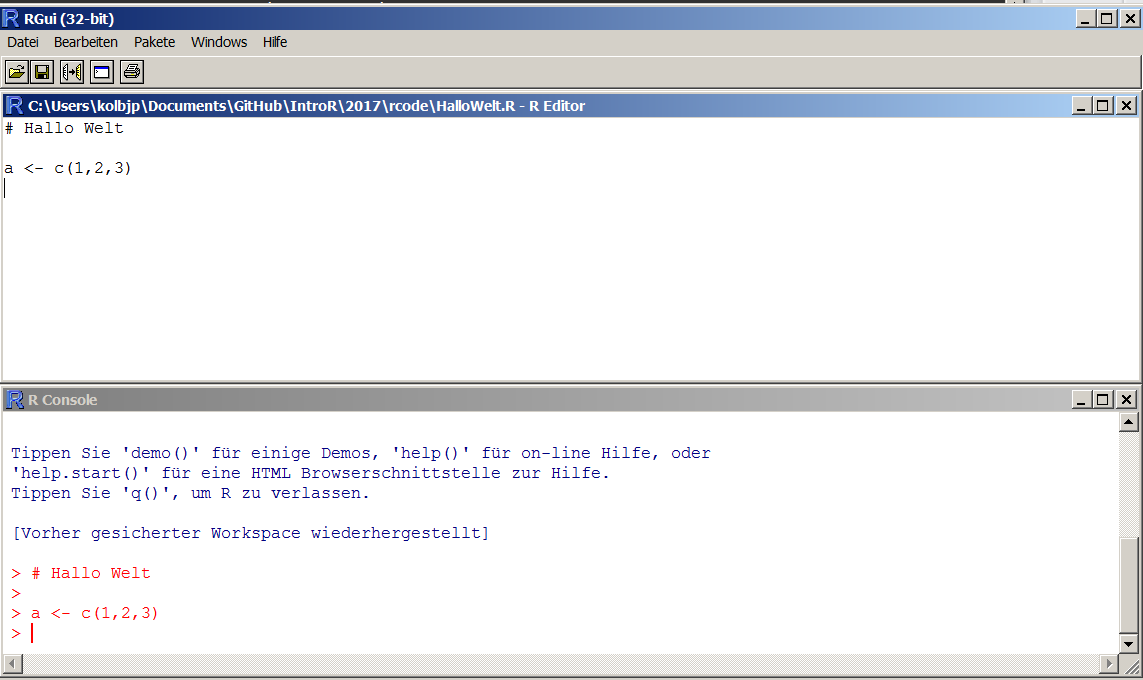
\includegraphics{figure/BasisR.PNG}

\end{block}

\end{frame}

\begin{frame}{Graphical user interface}
\protect\hypertarget{graphical-user-interface}{}

But many people use a graphical user interface (GUI) or a integrated
development interface (IDE).

For the following reasons:

\begin{itemize}
\tightlist
\item
  Syntax highlighting
\item
  Auto-completion
\item
  Better overview on graphics, libraries, files, \ldots{}
\end{itemize}

\end{frame}

\begin{frame}{Various text editors / IDEs}
\protect\hypertarget{various-text-editors-ides}{}

\begin{itemize}
\item
  \href{https://projects.gnome.org/gedit/}{\textbf{Gedit}} with
  R-specific Add-ons for Linux
\item
  \href{http://www.gnu.org/software/emacs/}{\textbf{Emacs}} and ESS
  (Emacs speaks statistics)- An extensible, customizable, free/libre
  text editor --- and more.
\item
  I use \href{https://www.rstudio.com/}{\textbf{Rstudio!}}
\end{itemize}

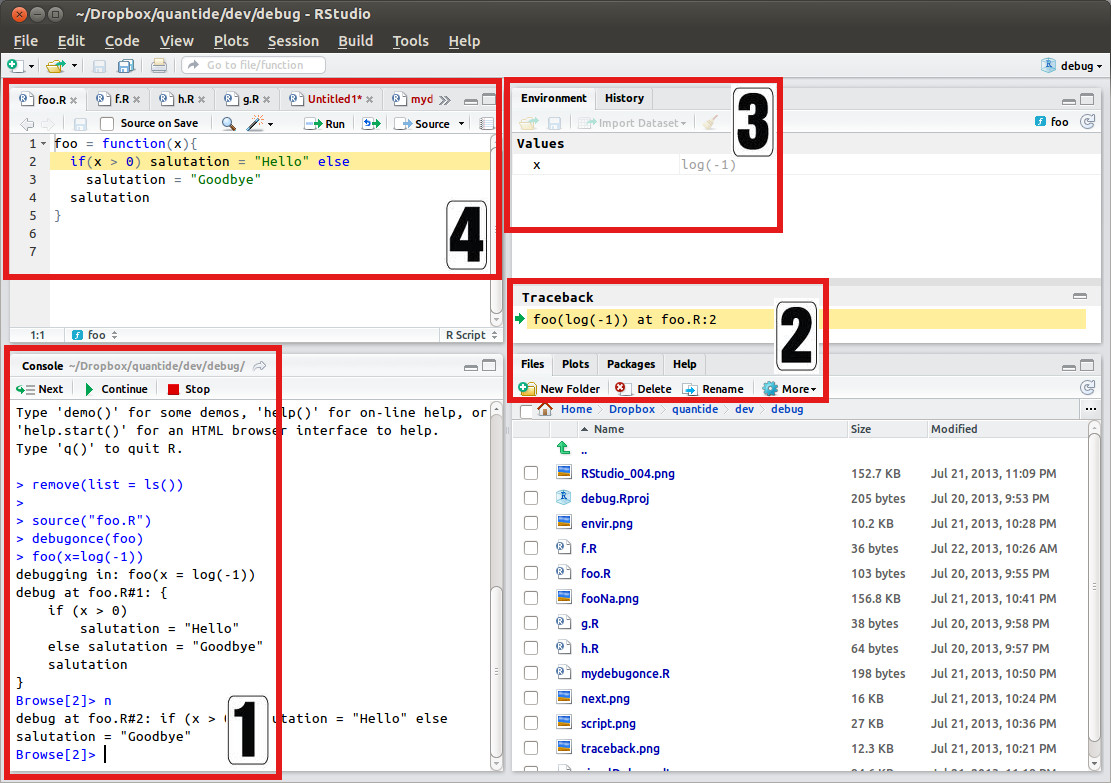
\includegraphics{figure/0_overall.jpg}

\end{frame}

\begin{frame}{\href{http://uc-r.github.io/introduction}{RStudio}}
\protect\hypertarget{rstudio}{}

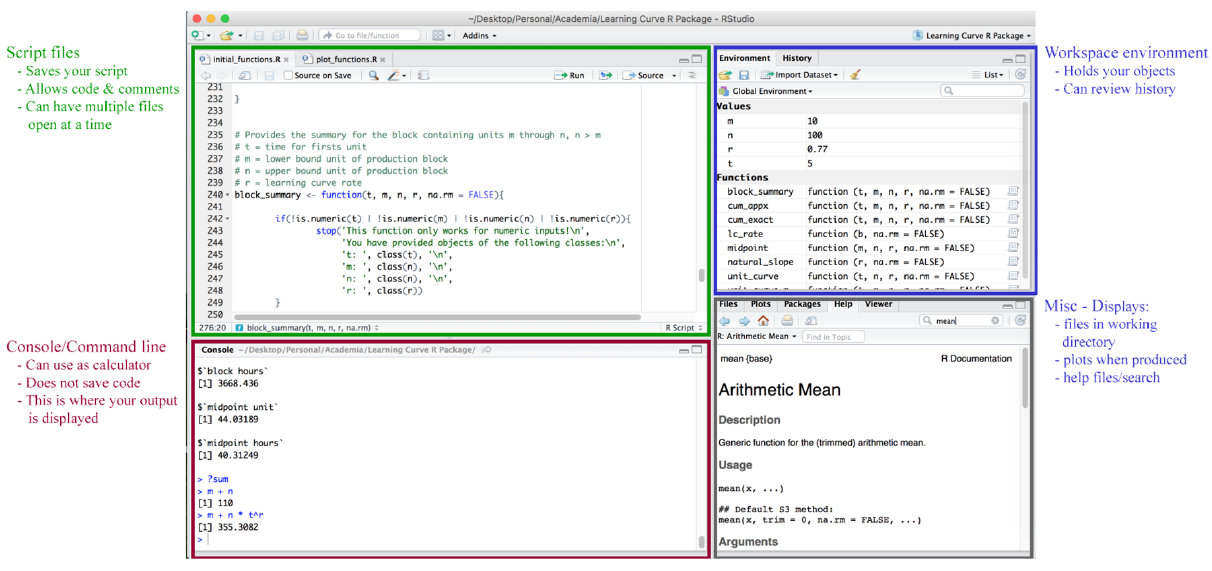
\includegraphics[width=1.1\textwidth,height=\textheight]{figure/rstudio_ide.PNG}

\end{frame}

\begin{frame}{Important Rstudio Buttons}
\protect\hypertarget{important-rstudio-buttons}{}


\includegraphics{figure/new_script.PNG} create a new script


\includegraphics{figure/Skriptoeffnen.PNG} open an existing script


\includegraphics{figure/runskript.PNG} run line where cursor is

\includegraphics{figure/find_replace.PNG} find and replace

\end{frame}

\begin{frame}[fragile]{R as a calculator}
\protect\hypertarget{r-as-a-calculator}{}

\begin{Shaded}
\begin{Highlighting}[]
\DecValTok{3} \OperatorTok{+}\StringTok{ }\DecValTok{2} \OperatorTok{/}\StringTok{ }\DecValTok{10}\OperatorTok{^}\DecValTok{2} \CommentTok{# Uses PEMDAS convention (order of operations)}
\end{Highlighting}
\end{Shaded}

\begin{verbatim}
## [1] 3.02
\end{verbatim}

\begin{Shaded}
\begin{Highlighting}[]
\DecValTok{3} \OperatorTok{+}\StringTok{ }\NormalTok{(}\DecValTok{2} \OperatorTok{/}\StringTok{ }\DecValTok{10}\OperatorTok{^}\DecValTok{2}\NormalTok{)}
\end{Highlighting}
\end{Shaded}

\begin{verbatim}
## [1] 3.02
\end{verbatim}

\begin{Shaded}
\begin{Highlighting}[]
\NormalTok{(}\DecValTok{3} \OperatorTok{+}\StringTok{ }\DecValTok{2}\NormalTok{) }\OperatorTok{/}\StringTok{ }\DecValTok{10}\OperatorTok{^}\DecValTok{2}
\end{Highlighting}
\end{Shaded}

\begin{verbatim}
## [1] 0.05
\end{verbatim}

\begin{Shaded}
\begin{Highlighting}[]
\DecValTok{1} \OperatorTok{/}\DecValTok{19}\OperatorTok{^}\DecValTok{4} \CommentTok{# scientific notation is used for large numbers}
\end{Highlighting}
\end{Shaded}

\begin{verbatim}
## [1] 7.67336e-06
\end{verbatim}

\begin{Shaded}
\begin{Highlighting}[]
\DecValTok{1}\OperatorTok{/}\DecValTok{0} \CommentTok{# Undefined calculations}
\end{Highlighting}
\end{Shaded}

\begin{verbatim}
## [1] Inf
\end{verbatim}

\begin{Shaded}
\begin{Highlighting}[]
\OtherTok{Inf} \OperatorTok{-}\StringTok{ }\OtherTok{Inf}
\end{Highlighting}
\end{Shaded}

\begin{verbatim}
## [1] NaN
\end{verbatim}

\end{frame}

\begin{frame}[fragile]{Exercise: Preparation}
\protect\hypertarget{exercise-preparation}{}

\begin{itemize}
\tightlist
\item
  Check if R is installed on your computer.
\item
  If not, download \href{r-project.org}{\textbf{R}} and install it.
\item
  Check if Rstudio is installed.
\item
  If not - \href{http://www.rstudio.com/}{\textbf{install}} Rstudio.
\item
  Start RStudio. Go to the console (lower left window) and write
\end{itemize}

\begin{Shaded}
\begin{Highlighting}[]
\DecValTok{3}\OperatorTok{+}\DecValTok{2}
\end{Highlighting}
\end{Shaded}

\begin{itemize}
\tightlist
\item
  If there is not already an editor open in the upper left window, then
  go to the file menu and open a new script. Check the date with
  \texttt{date()} and the R version with \texttt{sessionInfo()}.
\end{itemize}

\begin{Shaded}
\begin{Highlighting}[]
\KeywordTok{date}\NormalTok{()}
\end{Highlighting}
\end{Shaded}

\begin{Shaded}
\begin{Highlighting}[]
\KeywordTok{sessionInfo}\NormalTok{()}
\end{Highlighting}
\end{Shaded}

\end{frame}

\begin{frame}[fragile]{Exercise: See where things happen}
\protect\hypertarget{exercise-see-where-things-happen}{}

\begin{itemize}
\tightlist
\item
  Create a new \texttt{.R} script named \texttt{my\_first\_script.R}
\item
  Write and execute the following code in the \texttt{.R} script and
  identify where in Rstudio the outputs can be found.
\end{itemize}

\begin{Shaded}
\begin{Highlighting}[]
\NormalTok{mtcars}
\NormalTok{?sum}
\KeywordTok{hist}\NormalTok{(mtcars}\OperatorTok{$}\NormalTok{mpg)}
\NormalTok{random_numbers <-}\StringTok{ }\KeywordTok{runif}\NormalTok{(}\DecValTok{40}\NormalTok{)}
\KeywordTok{history}\NormalTok{()}
\end{Highlighting}
\end{Shaded}

\end{frame}

\begin{frame}[fragile]{R is a object-orientiented language}
\protect\hypertarget{r-is-a-object-orientiented-language}{}

\begin{block}{Vectors and assignments}

\begin{itemize}
\tightlist
\item
  R is a object-orientiented language
\item
  \texttt{\textless{}-} is the assignment operator
\end{itemize}

\begin{Shaded}
\begin{Highlighting}[]
\NormalTok{b <-}\StringTok{ }\KeywordTok{c}\NormalTok{(}\DecValTok{1}\NormalTok{,}\DecValTok{2}\NormalTok{) }\CommentTok{# create an object with the numbers 1 and 2}
\end{Highlighting}
\end{Shaded}

\begin{itemize}
\tightlist
\item
  A function can be applied to this object:
\end{itemize}

\begin{Shaded}
\begin{Highlighting}[]
\KeywordTok{mean}\NormalTok{(b) }\CommentTok{# computes the mean}
\end{Highlighting}
\end{Shaded}

\begin{verbatim}
## [1] 1.5
\end{verbatim}

We can learn something about the properties of the object:

\begin{Shaded}
\begin{Highlighting}[]
\KeywordTok{length}\NormalTok{(b) }\CommentTok{# b has the length 2}
\end{Highlighting}
\end{Shaded}

\begin{verbatim}
## [1] 2
\end{verbatim}

\begin{Shaded}
\begin{Highlighting}[]
\KeywordTok{sqrt}\NormalTok{(b) }\CommentTok{# the square root of b}
\end{Highlighting}
\end{Shaded}

\begin{verbatim}
## [1] 1.000000 1.414214
\end{verbatim}

\end{block}

\end{frame}

\begin{frame}{Functions in base-package}
\protect\hypertarget{functions-in-base-package}{}

\begin{longtable}[]{@{}lll@{}}
\toprule
Function & Meaning & Example\tabularnewline
\midrule
\endhead
str() & Object structure & str(b)\tabularnewline
max() & Maximum & max(b)\tabularnewline
min() & Minimum & min(b)\tabularnewline
sd() & Standard deviation & sd(b)\tabularnewline
var() & Variance & var(b)\tabularnewline
mean() & Mean & mean(b)\tabularnewline
median() & Median & median(b)\tabularnewline
\bottomrule
\end{longtable}

These functions only need one argument.

\end{frame}

\begin{frame}[fragile]{Functions with more arguments}
\protect\hypertarget{functions-with-more-arguments}{}

\begin{block}{Other functions need more arguments:}

\begin{longtable}[]{@{}lll@{}}
\toprule
Argument & Meaning & Example\tabularnewline
\midrule
\endhead
quantile() & 90 \% Quantile & quantile(b,.9)\tabularnewline
sample() & Draw a sample & sample(b,1)\tabularnewline
\bottomrule
\end{longtable}

\begin{Shaded}
\begin{Highlighting}[]
\KeywordTok{quantile}\NormalTok{(b,.}\DecValTok{9}\NormalTok{)}
\end{Highlighting}
\end{Shaded}

\begin{verbatim}
## 90% 
## 1.9
\end{verbatim}

\begin{Shaded}
\begin{Highlighting}[]
\KeywordTok{sample}\NormalTok{(b,}\DecValTok{1}\NormalTok{) }
\end{Highlighting}
\end{Shaded}

\begin{verbatim}
## [1] 1
\end{verbatim}

\end{block}

\end{frame}

\begin{frame}[fragile]{Examples - Functions with more than one argument}
\protect\hypertarget{examples---functions-with-more-than-one-argument}{}

\begin{Shaded}
\begin{Highlighting}[]
\KeywordTok{max}\NormalTok{(b); }\KeywordTok{min}\NormalTok{(b)}
\end{Highlighting}
\end{Shaded}

\begin{verbatim}
## [1] 2
\end{verbatim}

\begin{verbatim}
## [1] 1
\end{verbatim}

\begin{Shaded}
\begin{Highlighting}[]
\KeywordTok{sd}\NormalTok{(b); }\KeywordTok{var}\NormalTok{(b)}
\end{Highlighting}
\end{Shaded}

\begin{verbatim}
## [1] 0.7071068
\end{verbatim}

\begin{verbatim}
## [1] 0.5
\end{verbatim}

\begin{block}{Functions with one argument}

\begin{Shaded}
\begin{Highlighting}[]
\KeywordTok{mean}\NormalTok{(b)}
\end{Highlighting}
\end{Shaded}

\begin{verbatim}
## [1] 1.5
\end{verbatim}

\begin{Shaded}
\begin{Highlighting}[]
\KeywordTok{median}\NormalTok{(b)}
\end{Highlighting}
\end{Shaded}

\begin{verbatim}
## [1] 1.5
\end{verbatim}

\end{block}

\end{frame}

\begin{frame}[fragile]{Exercise: Assignments and functions}
\protect\hypertarget{exercise-assignments-and-functions}{}

Create a vector \texttt{b} with the numbers from 1 to 5 and calculate
\ldots{}

\begin{enumerate}
\item
  the mean
\item
  the variance
\item
  the standard deviation
\item
  the square root from the mean
\end{enumerate}

\end{frame}

\begin{frame}{\href{http://cran.r-project.org/doc/manuals/R-intro.html}{\textbf{Overview
commands}}}
\protect\hypertarget{overview-commands}{}

\url{http://cran.r-project.org/doc/manuals/R-intro.html}

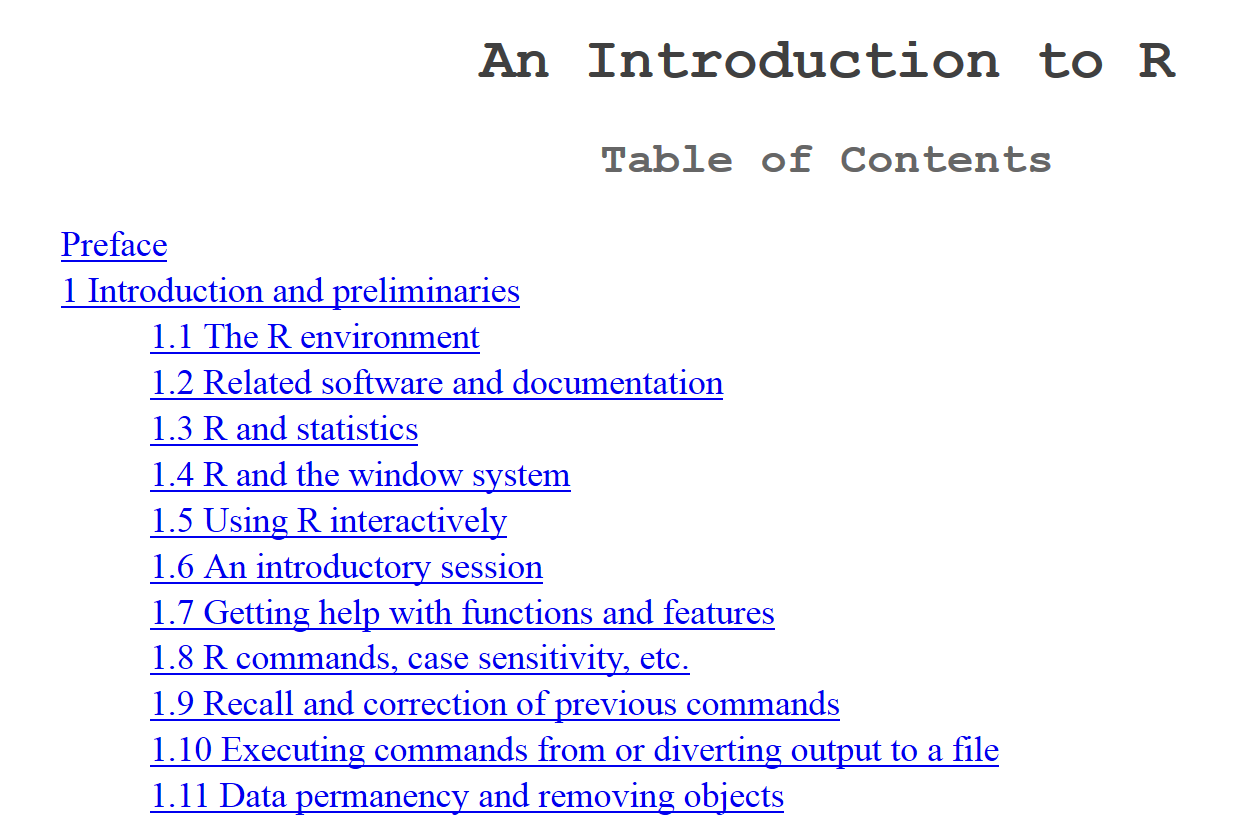
\includegraphics{figure/UebersichtBefehle.PNG}

\end{frame}

\begin{frame}{Exercise: Economic Order Quantity Model}
\protect\hypertarget{exercise-economic-order-quantity-model}{}

\begin{block}{Economic Order Quantity Model}

\[
Q = \sqrt{\dfrac{2DK}{h}}
\]

\end{block}

\begin{block}{Calculate \(Q\) where:}

\begin{itemize}
\tightlist
\item
  D = 1000
\item
  K = 5
\item
  h = 0.25
\end{itemize}

\end{block}

\end{frame}

\begin{frame}[fragile]{\href{https://www.stat.berkeley.edu/~nolan/stat133/Fall05/lectures/DataTypes4.pdf}{R
Data Types}}
\protect\hypertarget{r-data-types}{}

\begin{itemize}
\tightlist
\item
  R supports a few basic data types: integer, numeric, logical,
  character/string, factor, and complex
\end{itemize}

\begin{block}{Logical}

-- binary, two possible values represented by \texttt{TRUE} and
\texttt{FALSE}

\begin{Shaded}
\begin{Highlighting}[]
\NormalTok{x <-}\StringTok{ }\KeywordTok{c}\NormalTok{(}\DecValTok{3}\NormalTok{,}\DecValTok{7}\NormalTok{, }\DecValTok{1}\NormalTok{, }\DecValTok{2}\NormalTok{)}
\NormalTok{x }\OperatorTok{>}\StringTok{ }\DecValTok{2}
\end{Highlighting}
\end{Shaded}

\begin{verbatim}
## [1]  TRUE  TRUE FALSE FALSE
\end{verbatim}

\begin{Shaded}
\begin{Highlighting}[]
\NormalTok{x }\OperatorTok{==}\StringTok{ }\DecValTok{2}
\end{Highlighting}
\end{Shaded}

\begin{verbatim}
## [1] FALSE FALSE FALSE  TRUE
\end{verbatim}

\begin{Shaded}
\begin{Highlighting}[]
\OperatorTok{!}\NormalTok{(x }\OperatorTok{<}\StringTok{ }\DecValTok{3}\NormalTok{)}
\end{Highlighting}
\end{Shaded}

\begin{verbatim}
## [1]  TRUE  TRUE FALSE FALSE
\end{verbatim}

\begin{Shaded}
\begin{Highlighting}[]
\KeywordTok{which}\NormalTok{(x }\OperatorTok{>}\StringTok{ }\DecValTok{2}\NormalTok{)}
\end{Highlighting}
\end{Shaded}

\begin{verbatim}
## [1] 1 2
\end{verbatim}

\end{block}

\end{frame}

\begin{frame}[fragile]{\href{https://www.stat.berkeley.edu/~nolan/stat133/Fall05/lectures/DataTypes4.pdf}{Character
vectors}}
\protect\hypertarget{character-vectors}{}

\begin{Shaded}
\begin{Highlighting}[]
\NormalTok{y <-}\StringTok{ }\KeywordTok{c}\NormalTok{(}\StringTok{"a"}\NormalTok{,}\StringTok{"bc"}\NormalTok{,}\StringTok{"def"}\NormalTok{)}
\KeywordTok{length}\NormalTok{(y)}
\end{Highlighting}
\end{Shaded}

\begin{verbatim}
## [1] 3
\end{verbatim}

\begin{Shaded}
\begin{Highlighting}[]
\KeywordTok{nchar}\NormalTok{(y)}
\end{Highlighting}
\end{Shaded}

\begin{verbatim}
## [1] 1 2 3
\end{verbatim}

\begin{Shaded}
\begin{Highlighting}[]
\NormalTok{y }\OperatorTok{==}\StringTok{ "a"}
\end{Highlighting}
\end{Shaded}

\begin{verbatim}
## [1]  TRUE FALSE FALSE
\end{verbatim}

\begin{Shaded}
\begin{Highlighting}[]
\NormalTok{y }\OperatorTok{==}\StringTok{ "b"}
\end{Highlighting}
\end{Shaded}

\begin{verbatim}
## [1] FALSE FALSE FALSE
\end{verbatim}

\end{frame}

\begin{frame}[fragile]{Object structure}
\protect\hypertarget{object-structure}{}

\begin{Shaded}
\begin{Highlighting}[]
\KeywordTok{str}\NormalTok{(b) }\CommentTok{# b is a numeric vector}
\end{Highlighting}
\end{Shaded}

\begin{verbatim}
##  num [1:2] 1 2
\end{verbatim}

\begin{block}{Variable type \texttt{character}}

\begin{Shaded}
\begin{Highlighting}[]
\NormalTok{a <-}\StringTok{ }\NormalTok{letters}
\KeywordTok{length}\NormalTok{(letters)}
\end{Highlighting}
\end{Shaded}

\begin{verbatim}
## [1] 26
\end{verbatim}

\begin{Shaded}
\begin{Highlighting}[]
\NormalTok{a[}\DecValTok{1}\OperatorTok{:}\DecValTok{4}\NormalTok{]}
\end{Highlighting}
\end{Shaded}

\begin{verbatim}
## [1] "a" "b" "c" "d"
\end{verbatim}

\begin{Shaded}
\begin{Highlighting}[]
\KeywordTok{str}\NormalTok{(a)}
\end{Highlighting}
\end{Shaded}

\begin{verbatim}
##  chr [1:26] "a" "b" "c" "d" "e" "f" "g" "h" "i" "j" "k" "l" "m" "n" "o" "p" ...
\end{verbatim}

\end{block}

\end{frame}

\begin{frame}[fragile]{Problems with character vector}
\protect\hypertarget{problems-with-character-vector}{}

\begin{Shaded}
\begin{Highlighting}[]
\KeywordTok{mean}\NormalTok{(b)}
\end{Highlighting}
\end{Shaded}

\begin{verbatim}
## [1] 1.5
\end{verbatim}

\begin{Shaded}
\begin{Highlighting}[]
\NormalTok{(b1 <-}\StringTok{ }\KeywordTok{c}\NormalTok{(b,}\StringTok{"a"}\NormalTok{))}
\end{Highlighting}
\end{Shaded}

\begin{verbatim}
## [1] "1" "2" "a"
\end{verbatim}

\begin{Shaded}
\begin{Highlighting}[]
\KeywordTok{mean}\NormalTok{(b1)}
\end{Highlighting}
\end{Shaded}

\begin{verbatim}
## Warning in mean.default(b1): argument is not numeric or logical: returning NA
\end{verbatim}

\begin{verbatim}
## [1] NA
\end{verbatim}

\end{frame}

\begin{frame}[fragile]{Coercion}
\protect\hypertarget{coercion}{}

\begin{itemize}
\tightlist
\item
  All elements in a vector must be of the same type. R coerces the
  elements to a common type
\item
  \texttt{c(1.2,3,TRUE)} -- In this case all elements are coerced to
  numeric.
\end{itemize}

\begin{Shaded}
\begin{Highlighting}[]
\NormalTok{x <-}\StringTok{ }\KeywordTok{c}\NormalTok{(}\OtherTok{TRUE}\NormalTok{,}\OtherTok{FALSE}\NormalTok{,}\OtherTok{TRUE}\NormalTok{)}
\KeywordTok{c}\NormalTok{(}\FloatTok{1.2}\NormalTok{,x)}
\end{Highlighting}
\end{Shaded}

\begin{verbatim}
## [1] 1.2 1.0 0.0 1.0
\end{verbatim}

\begin{Shaded}
\begin{Highlighting}[]
\NormalTok{y <-}\StringTok{ }\KeywordTok{c}\NormalTok{(}\StringTok{"2"}\NormalTok{,}\StringTok{"3"}\NormalTok{,}\StringTok{".2"}\NormalTok{)}
\KeywordTok{c}\NormalTok{(}\FloatTok{1.2}\NormalTok{,y, x)}
\end{Highlighting}
\end{Shaded}

\begin{verbatim}
## [1] "1.2"   "2"     "3"     ".2"    "TRUE"  "FALSE" "TRUE"
\end{verbatim}

\begin{itemize}
\tightlist
\item
  Sometimes this coercion occurs to perform an arithmetic operation:
\end{itemize}

\begin{Shaded}
\begin{Highlighting}[]
\DecValTok{1} \OperatorTok{+}\StringTok{ }\NormalTok{x}
\end{Highlighting}
\end{Shaded}

\begin{verbatim}
## [1] 2 1 2
\end{verbatim}

\end{frame}

\begin{frame}[fragile]{Perform the coercion}
\protect\hypertarget{perform-the-coercion}{}

\begin{itemize}
\tightlist
\item
  Other times we need to perform the coercion
\end{itemize}

\begin{Shaded}
\begin{Highlighting}[]
\KeywordTok{c}\NormalTok{(}\FloatTok{1.2}\NormalTok{,y)}
\end{Highlighting}
\end{Shaded}

\begin{verbatim}
## [1] "1.2" "2"   "3"   ".2"
\end{verbatim}

\begin{Shaded}
\begin{Highlighting}[]
\KeywordTok{c}\NormalTok{(}\FloatTok{1.2}\NormalTok{,}\KeywordTok{as.numeric}\NormalTok{(y))}
\end{Highlighting}
\end{Shaded}

\begin{verbatim}
## [1] 1.2 2.0 3.0 0.2
\end{verbatim}

\end{frame}

\begin{frame}[fragile]{Information about Vectors}
\protect\hypertarget{information-about-vectors}{}

\begin{itemize}
\item
  Aggregator functions - \texttt{sum}, \texttt{mean}, \texttt{range},
  \texttt{min}, \texttt{max}, \texttt{summary}, \texttt{table},
  \texttt{cut}, \ldots{}
\item
  \texttt{class(x)} -- returns the type of an object.
\item
  \texttt{is.logical(x)} -- tells us whether the object is a logical
  type. There is also \texttt{is.numeric}, \texttt{is.character},
  \texttt{is.integer}
\item
  \texttt{is.null} -- determines whether an object is empty, i.e.~has no
  content. 'NULL' is used mainly to represent the lists with zero
  length, and is often returned by expressions and functions whose value
  is undefined.
\end{itemize}

\end{frame}

\begin{frame}[fragile]{Coerce objects from one to another}
\protect\hypertarget{coerce-objects-from-one-to-another}{}

\begin{itemize}
\tightlist
\item
  \texttt{as.numeric(x)} -- we use the as-type functions to coerce
  objects from one type (e.g.~logical) to another, in this case numeric.
\item
  There are several of these functions, including \texttt{as.integer},
  \texttt{as.character}, \texttt{as.logical} 
\end{itemize}

\begin{Shaded}
\begin{Highlighting}[]
\NormalTok{x <-}\StringTok{ }\KeywordTok{c}\NormalTok{(}\StringTok{"1"}\NormalTok{,}\DecValTok{2}\NormalTok{,}\StringTok{"one"}\NormalTok{,}\StringTok{"1plus"}\NormalTok{,}\StringTok{"2_and"}\NormalTok{)}
\KeywordTok{as.numeric}\NormalTok{(x)}
\end{Highlighting}
\end{Shaded}

\begin{verbatim}
## [1]  1  2 NA NA NA
\end{verbatim}

\end{frame}

\begin{frame}[fragile]{Data Frames}
\protect\hypertarget{data-frames}{}

A data frame is a collection of vectors - different columns can have
different modes (numeric, character, factor, etc.).

\begin{block}{Three example vectors}

\begin{Shaded}
\begin{Highlighting}[]
\NormalTok{d <-}\StringTok{ }\KeywordTok{c}\NormalTok{(}\DecValTok{1}\NormalTok{,}\DecValTok{2}\NormalTok{,}\DecValTok{3}\NormalTok{,}\DecValTok{4}\NormalTok{)}
\NormalTok{e <-}\StringTok{ }\KeywordTok{c}\NormalTok{(}\StringTok{"red"}\NormalTok{, }\StringTok{"white"}\NormalTok{, }\StringTok{"red"}\NormalTok{, }\OtherTok{NA}\NormalTok{)}
\NormalTok{f <-}\StringTok{ }\KeywordTok{c}\NormalTok{(}\OtherTok{TRUE}\NormalTok{,}\OtherTok{TRUE}\NormalTok{,}\OtherTok{TRUE}\NormalTok{,}\OtherTok{FALSE}\NormalTok{)}
\end{Highlighting}
\end{Shaded}

\end{block}

\begin{block}{Bind the example vectors together:}

\begin{Shaded}
\begin{Highlighting}[]
\NormalTok{mydata <-}\StringTok{ }\KeywordTok{data.frame}\NormalTok{(d,e,f)}
\end{Highlighting}
\end{Shaded}

\end{block}

\begin{block}{Give the columns some names}

\begin{Shaded}
\begin{Highlighting}[]
\KeywordTok{names}\NormalTok{(mydata) <-}\StringTok{ }\KeywordTok{c}\NormalTok{(}\StringTok{"ID"}\NormalTok{,}\StringTok{"Color"}\NormalTok{,}\StringTok{"Passed"}\NormalTok{) }\CommentTok{# variable names}
\end{Highlighting}
\end{Shaded}

\end{block}

\end{frame}

\begin{frame}[fragile]{Identify the elements of a data frame}
\protect\hypertarget{identify-the-elements-of-a-data-frame}{}

There are a variety of ways to identify the elements of a data frame .

\begin{Shaded}
\begin{Highlighting}[]
\NormalTok{myframe[}\DecValTok{3}\OperatorTok{:}\DecValTok{5}\NormalTok{] }\CommentTok{# columns 3,4,5 of data frame}
\NormalTok{myframe[}\KeywordTok{c}\NormalTok{(}\StringTok{"ID"}\NormalTok{,}\StringTok{"Age"}\NormalTok{)] }\CommentTok{# columns ID and Age from data frame}
\NormalTok{myframe}\OperatorTok{$}\NormalTok{X1 }\CommentTok{# variable x1 in the data frame }
\end{Highlighting}
\end{Shaded}

\end{frame}

\begin{frame}[fragile]{\href{https://www.statmethods.net/input/datatypes.html}{Matrices}}
\protect\hypertarget{matrices}{}

All columns in a matrix must have the same mode (numeric, character,
etc.) and the same length. The general format is:

\begin{Shaded}
\begin{Highlighting}[]
\CommentTok{# generates 5 x 4 numeric matrix}
\NormalTok{y <-}\StringTok{ }\KeywordTok{matrix}\NormalTok{(}\DecValTok{1}\OperatorTok{:}\DecValTok{20}\NormalTok{, }\DataTypeTok{nrow=}\DecValTok{5}\NormalTok{,}\DataTypeTok{ncol=}\DecValTok{4}\NormalTok{)}
\end{Highlighting}
\end{Shaded}

\begin{itemize}
\tightlist
\item
  \texttt{byrow=TRUE} indicates that the matrix should be filled by
  rows.
\item
  \texttt{byrow=FALSE} - matrix should be filled by columns (the
  default).
\end{itemize}

\begin{Shaded}
\begin{Highlighting}[]
\CommentTok{# an example}
\NormalTok{cells <-}\StringTok{ }\KeywordTok{c}\NormalTok{(}\DecValTok{1}\NormalTok{,}\DecValTok{26}\NormalTok{,}\DecValTok{24}\NormalTok{,}\DecValTok{68}\NormalTok{)}
\NormalTok{mymatrix <-}\StringTok{ }\KeywordTok{matrix}\NormalTok{(cells, }\DataTypeTok{nrow=}\DecValTok{2}\NormalTok{, }\DataTypeTok{ncol=}\DecValTok{2}\NormalTok{, }\DataTypeTok{byrow=}\OtherTok{TRUE}\NormalTok{) }
\end{Highlighting}
\end{Shaded}

\end{frame}

\begin{frame}[fragile]{Matrix - dimnames}
\protect\hypertarget{matrix---dimnames}{}

\begin{itemize}
\tightlist
\item
  \texttt{dimnames} provides optional labels for the columns and rows.
\end{itemize}

\begin{Shaded}
\begin{Highlighting}[]
\CommentTok{# another example}
\NormalTok{rnames <-}\StringTok{ }\KeywordTok{c}\NormalTok{(}\StringTok{"R1"}\NormalTok{, }\StringTok{"R2"}\NormalTok{)}
\NormalTok{cnames <-}\StringTok{ }\KeywordTok{c}\NormalTok{(}\StringTok{"C1"}\NormalTok{, }\StringTok{"C2"}\NormalTok{)}
\NormalTok{mymatrix <-}\StringTok{ }\KeywordTok{matrix}\NormalTok{(cells, }\DataTypeTok{nrow=}\DecValTok{2}\NormalTok{, }\DataTypeTok{ncol=}\DecValTok{2}\NormalTok{, }\DataTypeTok{byrow=}\OtherTok{TRUE}\NormalTok{,}
  \DataTypeTok{dimnames=}\KeywordTok{list}\NormalTok{(rnames, cnames)) }
\end{Highlighting}
\end{Shaded}

\end{frame}

\begin{frame}[fragile]{Matrices and subscripts}
\protect\hypertarget{matrices-and-subscripts}{}

Identify rows, columns or elements using subscripts.

\begin{Shaded}
\begin{Highlighting}[]
\NormalTok{x[,}\DecValTok{4}\NormalTok{] }\CommentTok{# 4th column of matrix}
\NormalTok{x[}\DecValTok{3}\NormalTok{,] }\CommentTok{# 3rd row of matrix}
\NormalTok{x[}\DecValTok{2}\OperatorTok{:}\DecValTok{4}\NormalTok{,}\DecValTok{1}\OperatorTok{:}\DecValTok{3}\NormalTok{] }\CommentTok{# rows 2,3,4 of columns 1,2,3 }
\end{Highlighting}
\end{Shaded}

\end{frame}

\begin{frame}[fragile]{Lists}
\protect\hypertarget{lists}{}

An ordered collection of objects (components). A list allows you to
gather a variety of (possibly unrelated) objects under one name.

\begin{Shaded}
\begin{Highlighting}[]
\CommentTok{# example of a list with 4 components -}
\CommentTok{# a string, a numeric vector, a matrix, and a scaler}
\NormalTok{w <-}\StringTok{ }\KeywordTok{list}\NormalTok{(}\DataTypeTok{name=}\StringTok{"Fred"}\NormalTok{, }\DataTypeTok{mynumbers=}\NormalTok{a, }\DataTypeTok{mymatrix=}\NormalTok{y, }\DataTypeTok{age=}\FloatTok{5.3}\NormalTok{)}

\CommentTok{# example of a list containing two lists}
\NormalTok{v <-}\StringTok{ }\KeywordTok{c}\NormalTok{(list1,list2)}
\end{Highlighting}
\end{Shaded}

Identify elements of a list using the {[}{[} {]}{]} convention.

\begin{Shaded}
\begin{Highlighting}[]
\NormalTok{mylist[[}\DecValTok{2}\NormalTok{]] }\CommentTok{# 2nd component of the list}
\NormalTok{mylist[[}\StringTok{"mynumbers"}\NormalTok{]] }\CommentTok{# component named mynumbers in list}
\end{Highlighting}
\end{Shaded}

\end{frame}

\begin{frame}{\href{https://stats.idre.ucla.edu/r/seminars/intro/}{\textbf{Where
to find routines}}}
\protect\hypertarget{where-to-find-routines}{}

\begin{itemize}
\tightlist
\item
  Many functions are included in basic R
\item
  Many specific functions are integrated in additional libraries
\item
  R can be modularly extended by so-called packages or libraries
\item
  Most important packages hosted on CRAN (15342 at Fr Jan 10)
\item
  Further packages can be found e.g.~at
  \href{www.bioconductor.org}{\textbf{bioconductor}}
\end{itemize}

\begin{block}{Overview R packages}

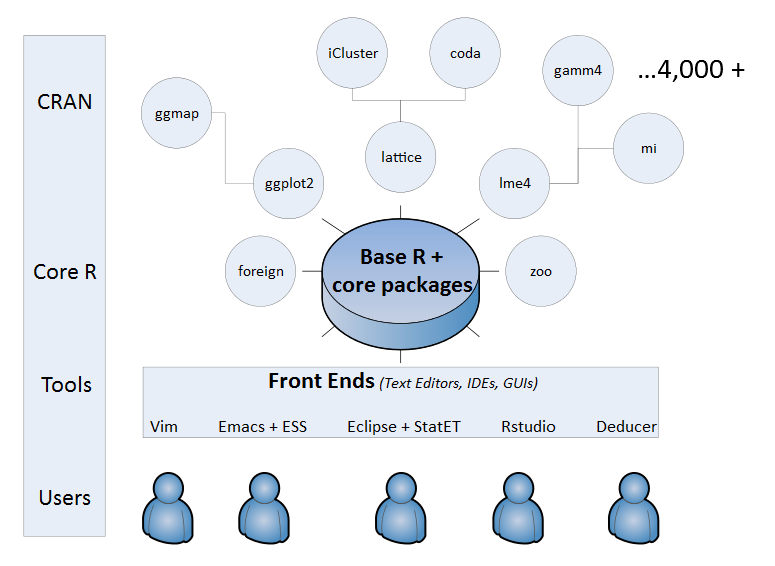
\includegraphics[width=\textwidth,height=0.6\textheight]{figure/Packages.PNG}

\end{block}

\end{frame}

\begin{frame}[fragile]{Installation of packages}
\protect\hypertarget{installation-of-packages}{}

\begin{itemize}
\tightlist
\item
  The quotes around the package name are necessary for the command
  \texttt{install.packages}.
\item
  They are optional for the command \texttt{library}.
\item
  You can also use \texttt{require} instead of \texttt{library}.
\end{itemize}

\begin{Shaded}
\begin{Highlighting}[]
\KeywordTok{install.packages}\NormalTok{(}\StringTok{"lme4"}\NormalTok{)}

\KeywordTok{library}\NormalTok{(lme4)}
\end{Highlighting}
\end{Shaded}

\end{frame}

\begin{frame}{Installation of packages with RStudio}
\protect\hypertarget{installation-of-packages-with-rstudio}{}

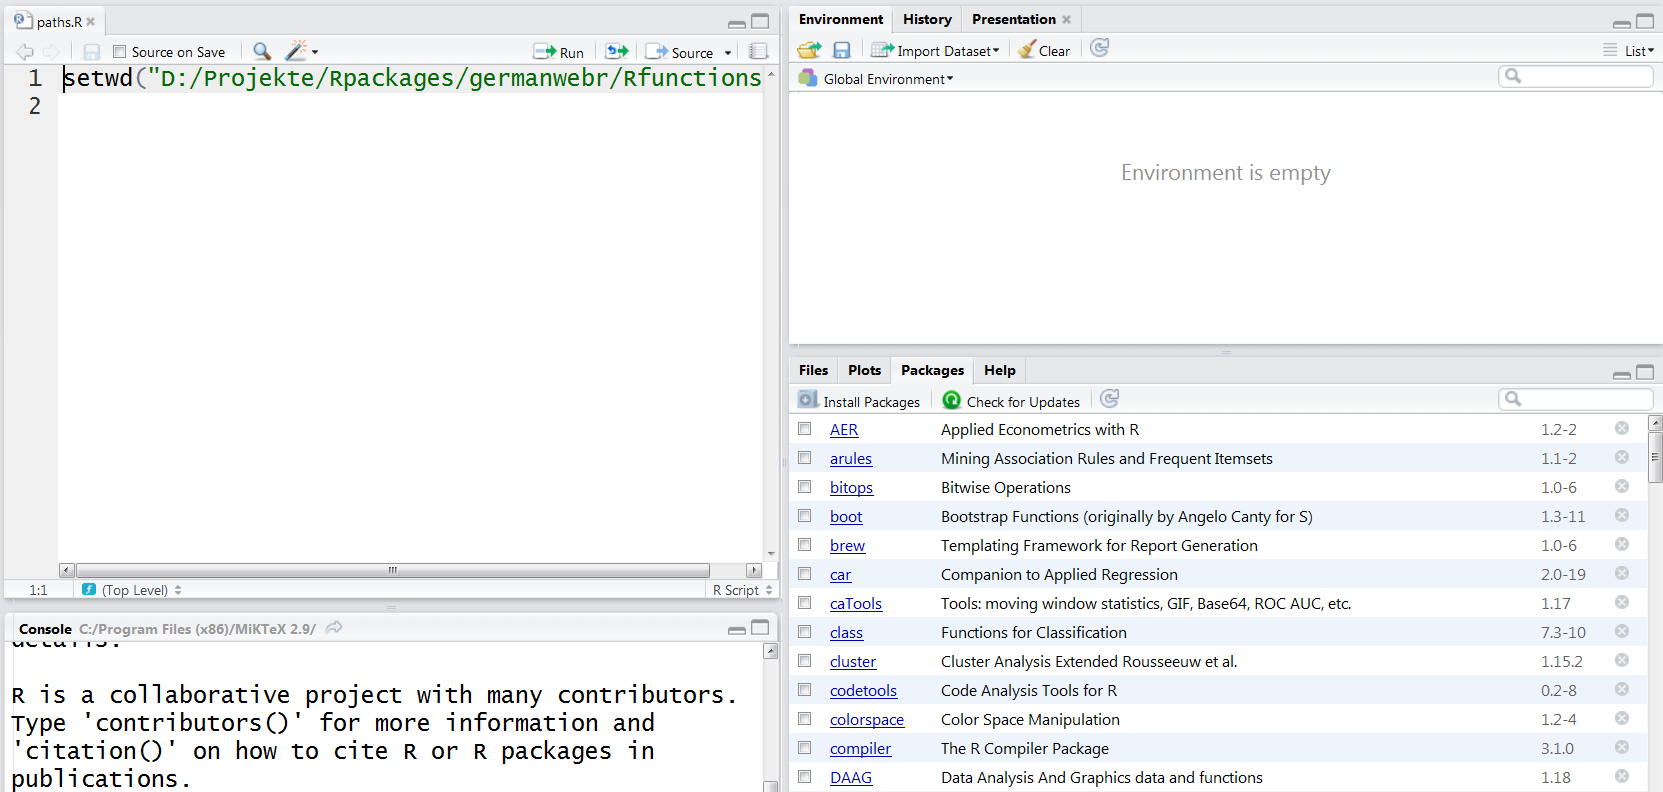
\includegraphics{figure/PaketeRstudio.PNG}

\end{frame}

\begin{frame}{Existing packages and installation}
\protect\hypertarget{existing-packages-and-installation}{}

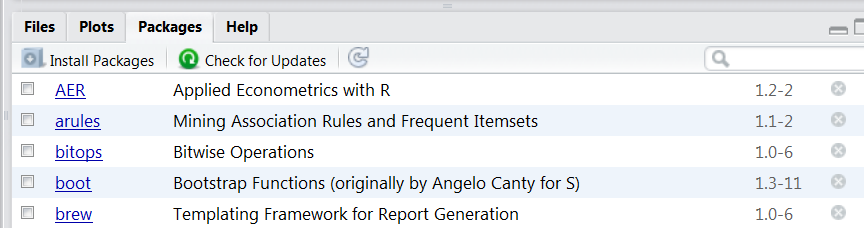
\includegraphics{figure/packages3.PNG}

\end{frame}

\begin{frame}[fragile]{Exercise: Download packages}
\protect\hypertarget{exercise-download-packages}{}

Download and install the following packages from CRAN:

\begin{itemize}
\tightlist
\item
  \texttt{tidyverse}
\item
  \texttt{nycflights13}
\item
  \texttt{cluster}
\item
  \texttt{ggplot2}
\item
  \texttt{tmap}
\end{itemize}

Have a look at the package documentation. What are these packages for?

\end{frame}

\begin{frame}[fragile]{Overview of many useful packages:}
\protect\hypertarget{overview-of-many-useful-packages}{}

\begin{itemize}
\tightlist
\item
  Luhmann -
  \href{http://www.beltz.de/fileadmin/beltz/downloads/OnlinematerialienPVU/28090_Luhmann/Verwendete\%20Pakete.pdf}{\textbf{Table
  with many useful packages}}
\end{itemize}

\begin{block}{Other interesting packages:}

\begin{itemize}
\item
  Package for Import/Export -
  \href{http://cran.r-project.org/web/packages/foreign/foreign.pdf}{\textbf{\texttt{foreign}}}
\item
  \href{http://iase-web.org/documents/papers/icots8/ICOTS8_4J1_TILLE.pdf}{\textbf{\texttt{sampling}-package
  for survey Sampling}}
\item
  \texttt{xtable} Package for integrating LateX in R
  (\href{http://cran.r-project.org/web/packages/xtable/vignettes/xtableGallery.pdf}{\textbf{xtable
  Galerie}})
\item
  \href{http://cran.r-project.org/web/packages/dummies/dummies.pdf}{\textbf{\texttt{dummies}
  package for creating dummies}}
\item
  \href{http://cran.r-project.org/web/packages/mvtnorm/index.html}{\textbf{Package
  \texttt{mvtnorm} for getting a multivariate normal distribution}}
\item
  \href{http://www.r-bloggers.com/tag/maptools/}{\textbf{Package
  \texttt{maptools} for creating maps}}
\end{itemize}

\end{block}

\end{frame}

\begin{frame}[fragile]{Install packages from various sources}
\protect\hypertarget{install-packages-from-various-sources}{}

\begin{block}{Install packages from CRAN Server}

\begin{Shaded}
\begin{Highlighting}[]
\KeywordTok{install.packages}\NormalTok{(}\StringTok{"lme4"}\NormalTok{)}
\end{Highlighting}
\end{Shaded}

\end{block}

\begin{block}{Install packages from Bioconductor Server}

\begin{Shaded}
\begin{Highlighting}[]
\KeywordTok{source}\NormalTok{(}\StringTok{"https://bioconductor.org/biocLite.R"}\NormalTok{)}
\KeywordTok{biocLite}\NormalTok{(}\KeywordTok{c}\NormalTok{(}\StringTok{"GenomicFeatures"}\NormalTok{, }\StringTok{"AnnotationDbi"}\NormalTok{))}
\end{Highlighting}
\end{Shaded}

\end{block}

\begin{block}{Install packages from Github}

\begin{Shaded}
\begin{Highlighting}[]
\KeywordTok{install.packages}\NormalTok{(}\StringTok{"devtools"}\NormalTok{)}
\KeywordTok{library}\NormalTok{(devtools)}

\KeywordTok{install_github}\NormalTok{(}\StringTok{"hadley/ggplot2"}\NormalTok{)}
\end{Highlighting}
\end{Shaded}

\end{block}

\end{frame}

\begin{frame}[fragile]{Packages}
\protect\hypertarget{packages}{}

\begin{Shaded}
\begin{Highlighting}[]
\CommentTok{# load the package to use in the current R session}
\KeywordTok{library}\NormalTok{(tidyverse)}

\CommentTok{# use a particular function within a package }
\CommentTok{# without loading the package}
\NormalTok{stringr}\OperatorTok{::}\KeywordTok{str_replace}\NormalTok{()}
\end{Highlighting}
\end{Shaded}

\begin{block}{Getting help on packages}

\begin{Shaded}
\begin{Highlighting}[]
\CommentTok{# provides details regarding contents of a package}
\KeywordTok{help}\NormalTok{(}\DataTypeTok{package =} \StringTok{"tidyr"}\NormalTok{)}
\CommentTok{# list vignettes available for a specific package}
\KeywordTok{vignette}\NormalTok{(}\DataTypeTok{package=}\StringTok{"tidyr"}\NormalTok{)}
\CommentTok{# view specific vignette}
\KeywordTok{vignette}\NormalTok{(}\StringTok{"tidy-data"}\NormalTok{)}
\end{Highlighting}
\end{Shaded}

\end{block}

\end{frame}

\begin{frame}{How do I get an overview}
\protect\hypertarget{how-do-i-get-an-overview}{}

\begin{itemize}
\item
  \href{https://mran.microsoft.com/packages/}{\textbf{Discover packages
  recently uploaded to CRAN}}
\item
  Look at the Shiny web app that shows the
  \href{https://gallery.shinyapps.io/cran-gauge/}{\textbf{packages
  recently downloaded from CRAN}}
\item
  Have a look at a
  \href{https://support.rstudio.com/hc/en-us/articles/201057987-Quick-list-of-useful-R-packages}{\textbf{quick-list
  of useful packages}},\ldots{}
\item
  \ldots{}, or at a list with the
  \href{http://www.computerworld.com/article/2921176/business-intelligence/great-r-packages-for-data-import-wrangling-visualization.html}{\textbf{best
  packages for data processing and analysis}},\ldots{}
\item
  \ldots{}, or at
  \href{https://www.r-bloggers.com/the-50-most-used-r-packages/}{\textbf{the
  50 most used packages}}
\end{itemize}

\end{frame}

\begin{frame}[fragile]{CRAN Task Views}
\protect\hypertarget{cran-task-views}{}

\begin{itemize}
\tightlist
\item
  For some topics all possibilities are arranged in R.
  (\href{https://cran.r-project.org/web/views/}{\textbf{Overview of Task
  Views}})
\item
  Currently there are 35 task views.
\item
  All packages of a task view can be installed with the following
  \href{https://mran.microsoft.com/rpackages/}{\textbf{command:}}
\end{itemize}

\begin{Shaded}
\begin{Highlighting}[]
\KeywordTok{install.packages}\NormalTok{(}\StringTok{"ctv"}\NormalTok{)}
\KeywordTok{library}\NormalTok{(}\StringTok{"ctv"}\NormalTok{)}
\KeywordTok{install.views}\NormalTok{(}\StringTok{"Bayesian"}\NormalTok{)}
\end{Highlighting}
\end{Shaded}

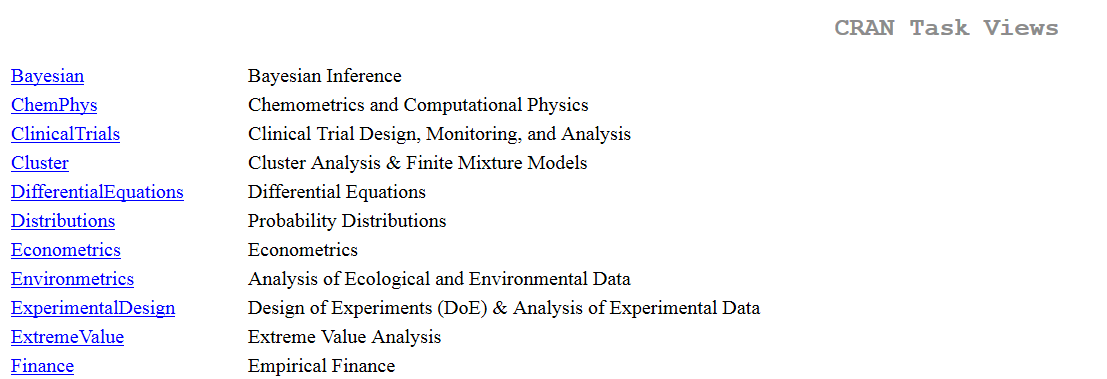
\includegraphics{figure/CRANtaskViews.PNG}

\end{frame}

\begin{frame}[fragile]{Exercise: additional packages}
\protect\hypertarget{exercise-additional-packages}{}

\begin{block}{Go for example to:}

\url{https://cran.r-project.org/}

\url{https://awesome-r.com/}

\end{block}

\begin{block}{or search for}

\begin{verbatim}
most interesting r packages
\end{verbatim}

\end{block}

\begin{block}{and search for packages \ldots{}}

\begin{itemize}
\tightlist
\item
  for descriptive data analysis.
\item
  with functions to work with date-times and time-spans.
\item
  to use an interface to \texttt{python}.
\item
  to import foreign data (e.g.~SPSS data).
\item
  to handle large amounts of data
\end{itemize}

\end{block}

\end{frame}

\begin{frame}{\href{https://lgatto.github.io/2017_11_09_Rcourse_Jena/before-we-start.html\#knowing-your-way-around-rstudio}{How
to learn after this workshop}}
\protect\hypertarget{how-to-learn-after-this-workshop}{}

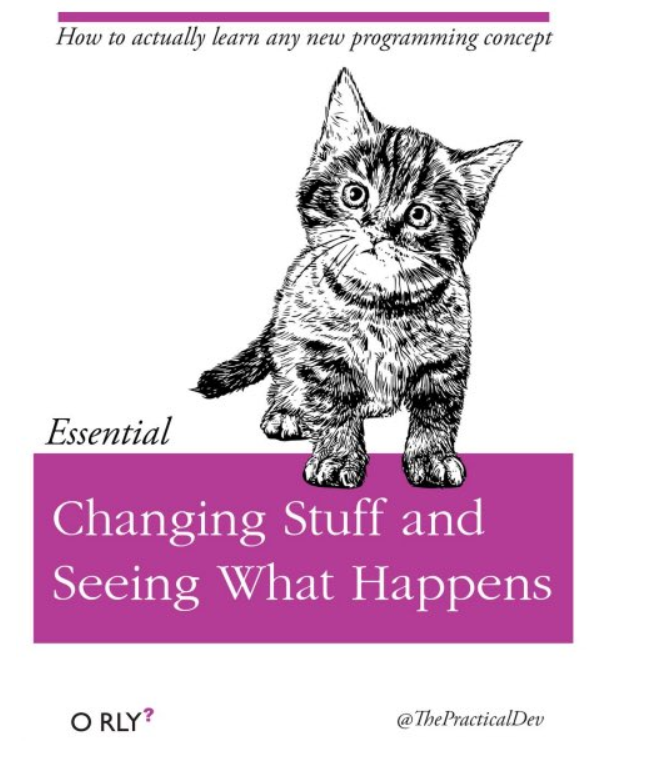
\includegraphics{figure/changing_stuff.PNG}

\end{frame}

\begin{frame}{Shiny App - Intro R}
\protect\hypertarget{shiny-app---intro-r}{}

\url{http://www.intro-stats.com/}

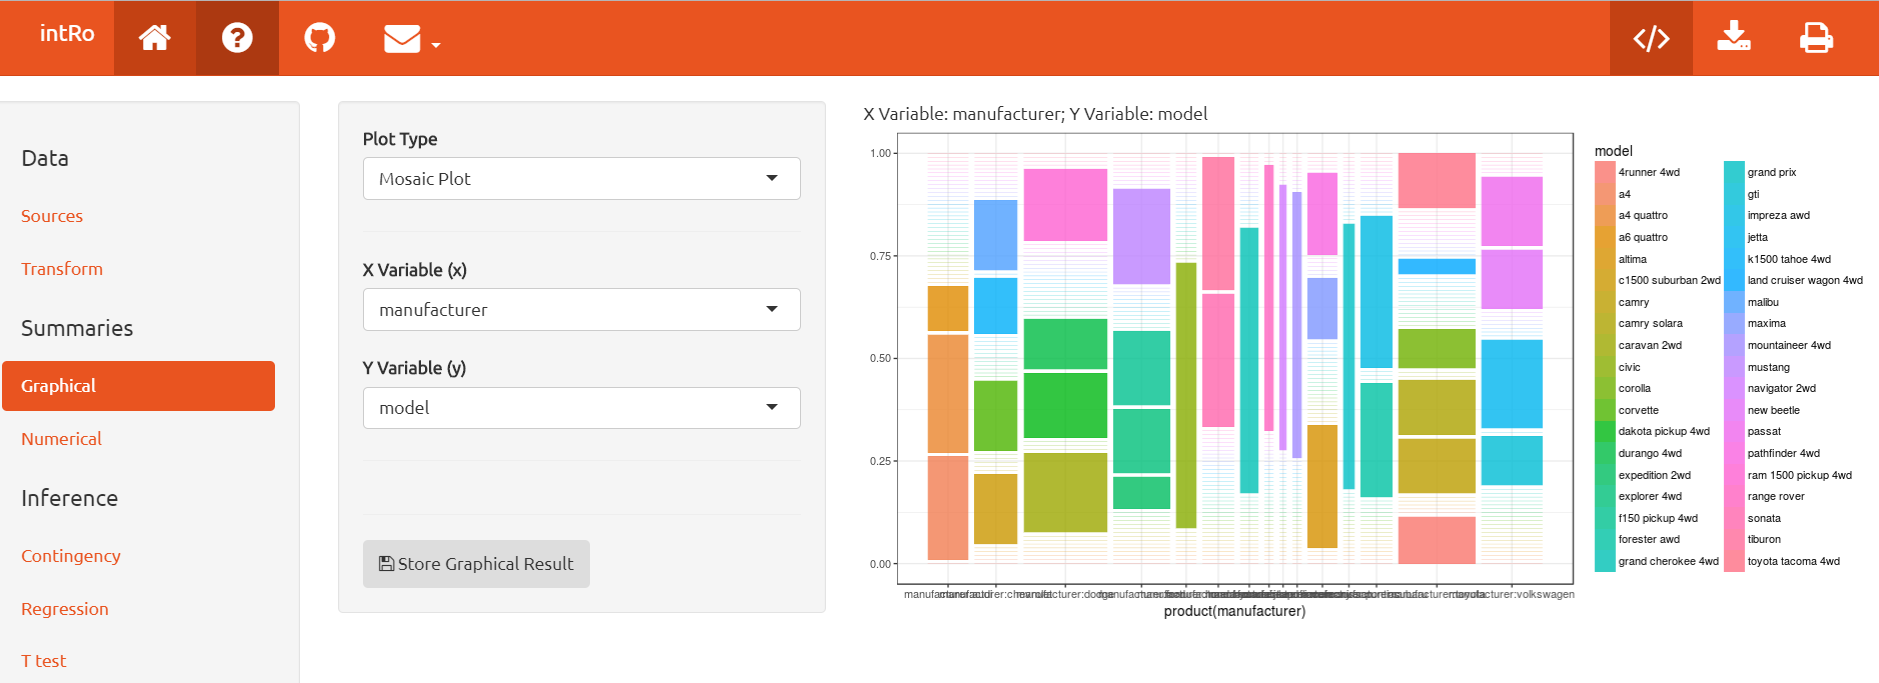
\includegraphics{figure/intror_shiny.PNG}

\end{frame}

\begin{frame}{Some links to read on}
\protect\hypertarget{some-links-to-read-on}{}

\begin{itemize}
\item
  Six
  \href{http://www.r-bloggers.com/top-6-reasons-you-need-to-be-using-rstudio/}{\textbf{reasons}}
  to use
  \href{https://support.rstudio.com/hc/en-us/articles/200549016-Customizing-RStudio}{\textbf{Rstudio}}.
\item
  \href{http://www.r-bloggers.com/why-you-should-learn-r-first-for-data-science/}{\textbf{Why
  you should learn R first for data science}}
\item
  \href{http://www.r-bloggers.com/rstudio-infoworld-2015-technology-of-the-year-award-recipient/}{\textbf{RStudio
  -- Infoworld 2015 Technology of the Year Award Recipient!}}
\item
  \href{http://www.fastcolabs.com/3030063/why\%20the\%20r\%20programming\%20language\%20is\%20good\%20for\%20business}{\textbf{Why
  the R programming language is good for business?}}
\item
  \href{http://www.r-bloggers.com/why-use-r/}{\textbf{Have a look at
  R-bloggers}} 
\item
  \href{http://www.dataschool.io/python-or-r-for-data-science/}{\textbf{Comparisson
  between python and R}}
\item
  \href{http://economistry.com/2013/11/r-impact-evaluation-r-stata-side-side/}{\textbf{R
  and Stata Side-by-side}}
\item
  \href{https://awesome-r.com/}{\textbf{AWESOME R}}
\item
  \href{https://support.bioconductor.org/p/33781/}{\textbf{1000 R
  tutorials/Links}}
\item
  \href{https://www.youtube.com/playlist?list=PLcgz5kNZFCkzSyBG3H-rUaPHoBXgijHfC}{\textbf{Learn
  R by watching two‐minute videos}}
\end{itemize}

\begin{block}{R for stata users}

\begin{itemize}
\tightlist
\item
  Oscar Torres-Reyna -
  \href{https://www.princeton.edu/~otorres/sessions/s2r.pdf}{\textbf{Exploring
  Data and Descriptive Statistics (using R)}}
\end{itemize}

\end{block}

\end{frame}

\end{document}
